\section{Label-Permutation Null Distributions (Supplementary)}
\label{app:perm_null}

Thirty label-shuffle fine-tuning runs per dataset, same LaBraM
recipe as the real runs. Each permutation shuffles recording-level
labels before subject-level StratifiedGroupKFold and yields one
subject-level BA draw.

\paragraph{Stress (contrast-bounded).} Real $0.443 \pm 0.083$
($n = 3$) falls inside null $0.506 \pm 0.063$ ($n = 30$; range
$0.393$--$0.661$; Fig.~\ref{fig:perm_null_density}, top). One-sided
Mann--Whitney $p \geq 0.5$. The $0.063$\,pp real-below-null offset
is within the $\pm 0.083$ seed envelope and is the expected
no-signal pattern under the sparse positive rate ($14/70$): with
only a handful of positive recordings, class-balanced FT on
shuffled labels has no coincidental subject-level alignment to
overfit, whereas real labels offer a per-seed pseudo-signal that
subject-held-out validation then rejects.

\paragraph{EEGMAT (anchored contrast).} Real $0.731 \pm 0.021$
exceeds every one of the thirty null draws (null
$0.498 \pm 0.053$; null max $0.611$;
Fig.~\ref{fig:perm_null_density}, bottom). Real minimum $0.714$
clears null maximum $0.611$ by $10.3$\,pp, so the permutation
$p$-value is below the $1/31 \approx 0.032$ floor.

The null means sit at $\approx 0.5$ on both cohorts, confirming
the permutation protocol carries no subject-leakage residual that
would bias chance upward.

\begin{figure}[!t]
\centering
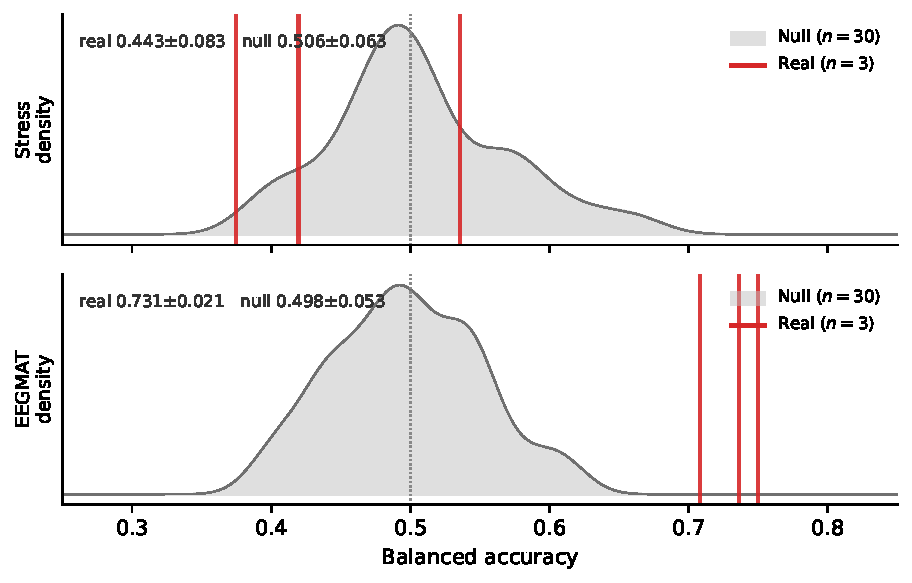
\includegraphics[width=0.9\linewidth]{figures/main/fig_perm_null_density.pdf}
\caption{Label-permutation null for LaBraM FT. Grey: thirty-permutation
  null kernel-density estimate. Red verticals: three real seeds.
  Dotted: chance ($0.50$). Stress (top) real sits inside the null
  support; EEGMAT (bottom) real sits entirely outside it.}
\label{fig:perm_null_density}
\end{figure}
